\section*{\textbf{April 18 (Sarah)}}
We've shown that $D$ is invertible in the special case $h_t=h$ is constant, and we've shown that $D$ is Fredholm in general. We still need to check that the index of $D$ is equal to the spectral flow of $L_0+h_t$. We'll only deal with two special cases.

\medskip

{\bf Case 1:} $h_t$ is hyperbolic for all $t$. By definition, the eigenvalues of $h_t$ never cross $i\R$, so the spectral flow is zero. To check $\Ind(D)=0$, we deform $D$ to something invertible. We define a family $D_s$ so that $D_0=\tfrac{d}{dt}+L_0+h_-$ and $D_1=D$.
\begin{center}
\begin{tikzpicture}[xscale=1.5]

\draw (-2,2.5) -- (2,2.5);
\node [above] at (0,2.5) {$L_0+h_-$};

\draw [->] (0,2) -- (0,1);

\draw (-2,0) -- (2,0);
\node at (-0.8,0) {$|$};
\node at (0.8,0) {$|$};
\node [below] at (-0.8,0) {$t_-$};
\node [below] at (0.8,0) {$t_0$};
\node [above] at (-1.5,0.1) {$L_0+h_-$};
\node [above] at (0,0.1) {$L_0+h_t$};
\node [above] at (1.5,0.1) {$L_0+h_{t_0}$};

\draw [->] (0,-0.5) -- (0,-1.5);

\draw (-2,-2.5) -- (2,-2.5);
\node at (-0.8,-2.5) {$|$};
\node at (0.8,-2.5) {$|$};
\node [below] at (-0.8,-2.5) {$t_-$};
\node [below] at (0.8,-2.5) {$t_+$};
\node [above] at (-1.5,-2.4) {$L_0+h_-$};
\node [above] at (0,-2.4) {$L_0+h_t$};
\node [above] at (1.5,-2.4) {$L_0+h_+$};

\end{tikzpicture}
\end{center}
In particular, this is a deformation through Fredholm operators, and since index is locally constant it follows that $\Ind(D)=\Ind(D_0)$. But $D_0$ is invertible, so the index is $0$.

\medskip

{\bf Case 2:} We assume that the spectrum of $L_0+h_t$ is simple (each eigenspace has dimension one) and $h_t$ are symmetric. Let $\lambda_1(t),\ldots,\lambda_n(t)$ be the eigenvalues which ever cross $0$, with eigenvectors $u_1(t),\ldots,u_n(t)$ (these eigenvectors are functions of $y$, but we'll ignore that to keep notation relatively simple). If we pick an appropriate basis, we can write
\[
D = \df{d}{dt} + \begin{pmatrix} \begin{array}{c|c}
A(t)
\\
\hline
& \lambda(t)
\end{array} \end{pmatrix},
\]
where
\[
\lambda(t) = \begin{pmatrix}
\lambda_1(t)
\\
& \ddots
\\
&& \lambda_n(t)
\end{pmatrix}
\]
and $A$ is some infinite-dimensional diagonal matrix. 

We now compute $\ker(D)$. Let $f \in \ker(D)$, and $f=c_1u_1+\ldots+c_nu_n$ for $c_1,\ldots,c_n$ functions of $t$. The argument below can be used to show that any $f \in \ker(D)$ has to be of this form as well.

We have
\begin{align*}
0 & = Df(t)
\\
& = \sumto{k=1}{n} \df{d}{dt}(c_k(t)u_k(t)) + (L_0+h_t)(c_k(t)u_k(t))
\\
& = \sumto{k=1}{n} \df{dc_k}{dt}(t)u_k(t) + c(t)\df{du}{dt}(t) + c_k(t)\lambda_k(t)u_k(t).
\end{align*}
But $\lambda_i$ and $u_i$ are constant at infinity (by hypothesis, $h_t$ is constant at infinity), so we can write
\[
\sumto{k=1}{n} \left( \df{dc_k}{dt}(t) + c_k(t)\lambda_k(\pm\oo) \right) u_k(\pm\oo) = 0
\]
for large enough $t$. Since $u_k(\pm\oo)$ are eigenvectors for $h_\pm$, they are linearly independent, which implies
\[
\df{dc}{dt}(t) + c_k(t)\lambda_k(\pm\oo) = 0
\]
for sufficiently large $t$. At $-\oo$, we get $c_k(t)=d_k^-e^{-\lambda_k(-\oo)t}$, and at $+\oo$ we have $c_k(t)=d_k^+e^{-\lambda_k(+\oo)t}$. In order for $f$ to be $L^2$, we need $\text{Re}(\lambda_k(-\oo))<0$ and $\text{Re}(\lambda_k(+\oo))>0$. Thus the dimension of $\ker(D)$ is the number of eigenvalues whose real part goes from negative to positive, which is precisely the number of intersections which count positively toward spectral flow.

A similar analysis will show that the dimension of $\coker(D)$ is the number of intersections which count negatively toward spectral flow. The basic idea is that we can define some kind of adjoint:
\[
D^* = -\df{d}{dt} + L_0 + h_t^*.
\]
Then the dimension of $\coker(D)$ is the dimension of $\ker(D^*)$, so we only need to relate $\ker(D^*)$ to the spectral flow. The relationship of elements of $\ker(D^*)$ to changes in signs of eigenvectors is nearly identical to the argument above, except that some signs are switched. Thus we add to the dimension of $\ker(D^*)$ when eigenvalues cross negatively. This completes the proof of case 2.

\medskip

\begin{remark} To see that the spectral index is finite, we need to note that the imaginary parts of the eigenvalues are bounded by the $L^2$ operator norm of $h-h^*$. We know that the norms of $h_t-h_t^*$ are uniformly bounded by continuity and compactness. Hence the eigenvalues in the spectral flow are contained in a band, finite in the imaginary direction. It then follows from the spectral theorem and basic principles of generic deformation that we can deform $D$ to something which fits into case 2, up to the assumption that $h_t$ is symmetric, which is probably not necessary for the argument.
\end{remark}

\bigskip

We now proceed to a case which is of special interest in symplectic geometry. In what follows, we use $(s,t)$ coordinates in $\R \times S^1$. We consider operators $D:L_1^2(\R \times S^1, \R^{2n}) \arr L^2(\R \times S^1, \R^{2n})$ of the form 
\[
D = \df{\partial}{\partial s} + J_0 \df{\partial}{\partial t} + S,
\]
where $J_0$ is the standard complex structure on $\R^{2n}$ and $S=S(s,t)$ is a smooth family of symmetric matrices satisfying
\[
\df{\partial S}{\partial s}(s,t) = 0
\]
for $|s| \gg 1$. We will see later that these operators arise as linearizations of the Floer equation.

We endow $\R^{2n}$ with the standard symplectic form $\omega_{st} = \langle \cdot, J_0 \cdot \rangle$. Let $Sp(2n)$ denote the Lie group of symplectic matrices, allow with a map $sp(2n) \xrightarrow{\sim} \text{Symm}$, $A \mapsto J_0A$. By integrating $S(s,t)$ in the $t$-direction we obtain a map $\Psi: \R \times \R \arr Sp(2n)$ such that
\[
\df{d\Psi}{dt} = J_0 S \Psi \qquad \text{and} \qquad \Psi(s,0) = I.
\]
Then there is some $T$ such that $\Psi(-s,t)=\Psi(-T,t)$ and $\Psi(s,t)=\Psi(T,t)$ for all $s>T$.
\begin{center}
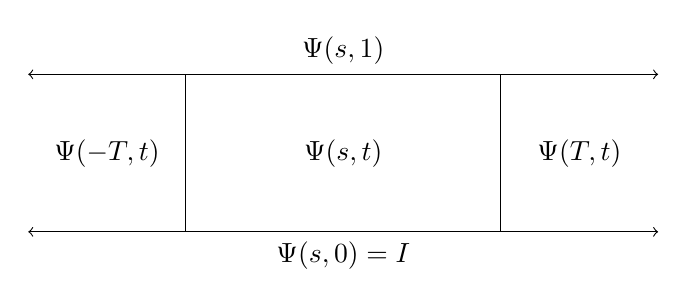
\begin{tikzpicture}

\draw [<->] (-4,0) -- (4,0);
\draw [<->] (-4,2) -- (4,2);

\draw (-2,0) -- (-2,2);
\draw (2,0) -- (2,2);

\node at (-3,1) {$\Psi(-T,t)$};
\node at (0,1) {$\Psi(s,t)$};
\node at (3,1) {$\Psi(T,t)$};

\node [below] at (0,0) {$\Psi(s,0)=I$};
\node [above] at (0,2) {$\Psi(s,1)$};

\end{tikzpicture}
\end{center}
Let $\gamma:[0,1]\arr Sp(2n)$ be a path such that $\gamma(0)=I$ and $1$ is not an eigenvalue of $\gamma(1)$. Then we can define a Maslov (or Conley-Zehnder) index $\mu_{CZ}(\gamma) \in \Z$. There are two ways to define it:
\begin{enumerate}[(1)]
\item Let $Sp^*(2n)$ be the set of symplectic matrices for which $1$ is not an eigenvalue. The Maslov cycle $Sp(2n) \setminus Sp^*(2n)$ is a singular codimension one subset, with singularities in codimension two.
\begin{center}
\begin{tikzpicture}[yscale=0.5]

\begin{scope}
    \clip (-2,0) rectangle (2,2);
    \draw [dashed] (0,0) ellipse (10mm and 4mm);
\end{scope}

\begin{scope}
    \clip (-2,0) rectangle (2,-2);
    \draw (0,0) ellipse (10mm and 4mm);
\end{scope}

\draw (-2,2) to [out=-45,in=105] (-1,0) to [out=-75,in=100] (0,-5) to [out=80,in=-105] (1,0) to [out=75,in=-135] (2,2);

\node at (0,-5) {$\bullet$};

\end{tikzpicture}
\end{center}
The Maslov cycle is co-orientable, which means that any transverse crossing of it can be given a sign. Then we can define $\mu_{CZ}$ to be the signed count of intersections with the Maslov cycle, for generic $\gamma$.

\item $Sp^*(2n)$ has two connected components; the component in which $M$ lies is determined by the sign of $\det(I-M)$. We identify a special point in each of these, $B_+=-I$ and
\[
B_- = \begin{pmatrix}
2
\\
& \tfrac12
\\
&& -1
\\
&&& \ddots
\\
&&&& -1
\end{pmatrix}.
\]
Any path $\gamma$ with $\gamma(1) \in Sp^*(2n)$ can be completed to a path $\tilde{\gamma}$ such that $\tilde{\gamma} \setminus \gamma$ doesn't cross the Maslov cycle and $\tilde{\gamma}(1) = B_\pm$.

We know $U(n)=Sp(2n) \cap O(2n)$, and $U(n)$ is a maximal compact subgroup of $Sp(2n)$. Inclusion is a homotopy equivalence. If $\rho:Sp(2n) \arr U(n)$ is a homotopy inverse to inclusion (in particular we use the one given by the polar decomposition of matrices in $Sp(2n)$), then $\det^2 \circ \rho \circ \tilde{\gamma}$ is a loop in $S^1$. Note that the $det$ here is the complex determinant of matrices in $U(n)$, its absolute value squared gives the real determinant. If we fix an isomorphism $\pi_1(S^1,1) \cong \Z$, we can define $\mu_{CZ}(\gamma) = [\det^2 \circ \rho \circ \tilde{\gamma}]$.
\end{enumerate}

The determinant map yields an isomorphism $\pi_1(Sp(2n),I) \arr \pi_1(S^1,1)$. If $\gamma(1)=I$, we can define $\mu_{CZ}(\gamma)=2[\gamma]_{\pi_1}$. In particular, if $\gamma$ is contractible then $\mu_{CZ}(\gamma)=0$.